\documentclass[letterpaper,12pt,twocolumn]{article}

\usepackage[subtle,margins]{savetrees}
%\usepackage[moderate,margins]{savetrees}
%\usepackage[extreme]{savetrees}
\usepackage{xspace}
\usepackage[inline]{enumitem}
\usepackage{graphicx}
\usepackage{anyfontsize}
\usepackage{sectsty}
\usepackage{amssymb}
\usepackage{amsthm}
\usepackage{amsmath}
\usepackage{booktabs}

\sectionfont{\fontsize{13}{18}\selectfont}

\newcommand\lspace{\hspace{-0.5em}}

\DeclareMathOperator{\splt}{split}
\DeclareMathOperator{\range}{range}

\newcommand\etal{\textit{et al.}\xspace}

\newcommand{\BigOh}[1]{O\!\left(#1\right)}
\newcommand\IR{\mathbb{R}}
\newcommand\D[1]{$D_{#1}$}
\newcommand\bounds[1]{[#1]}
\newcommand\lbounds[1]{(#1]} %chktex 9
\newcommand\rbounds[1]{[#1)} %chktex 9
\newcommand\lrbounds[1]{(#1)}

\theoremstyle{plain}
\newtheorem{theorem}{Theorem}

\begin{document}

{\noindent\Large 5-Sided Orthogonal Point Enclosure}\\
{\noindent Notes on Rahul 2015, by Simon Pratt}

The primary intention of these notes is to answer: how
does~\cite{saladi2015improved} answer 3D 5-sided point enclosure
queries?

\paragraph{Orthogonal Point Enclosure Queries (OPEQ)}
Preprocess a set $S$ of $n$ axes-parallel rectangles in $\IR^3$ in
order to determine all rectangles containing a query point $q$.  In
particular, we wish to consider the case in which a rectangle is
5-sided.  To be precise, our rectangles are of the form
$\bounds{x_1,x_2} \times \bounds{y_1, y_2} \times
\lbounds{-\infty,z}$.  In these notes, we will prove the following:

\begin{theorem}[5.1 in~\cite{saladi2015improved}]\label{thm:51}

  OPEQ on 5-sided rectangles can be answered using a structure of
  $\BigOh{n\lg^* n}$ size and $\BigOh{\lg n \lg\lg n + k}$ query time,
  where $k$ is the size of the output.

\end{theorem}

At a high level, we will use interval trees to solve 5-sided queries
in $\BigOh{\lg^3 n + k}$ time, which is good for $k \ge \lg^3 n$.
Otherwise, we'll use grids to break the structure into 4-sided queries
which we solve with $\BigOh{n\lg^* n}$ space and $\BigOh{\lg n\lg^* n
  + k}$ query time using interval trees, shallow cuttings, and the
following results:

\noindent\begin{tabular}{lccr}
    \toprule
    Problem & Query & Space & Reference \\
    \midrule
    %1D 2-sided OPEQ & $\BigOh{\lg n + k}$ & $\BigOh{n}$ & \cite{edelsbrunner1983new} \\ %chktex 2
    2D 4-sided OPEQ & $\BigOh{\lg n + k}$ & $\BigOh{n}$ & \cite{chazelle1986filtering} \\ %chktex 2
    3D 3-sided OPEQ & $\BigOh{\lg n + k}$ & $\BigOh{n}$ & \cite{afshani2008dominance} \\ %chktex 2
    \bottomrule
\end{tabular}

\section{\lspace{} 5-Sided: Slow/Simple with Linear Space}
\label{sec:slow}

An \emph{interval tree} is a binary tree whose leaves store the values
of the endpoints of a set of intervals~\cite{edelsbrunner1983new}.  At
each node $v$, store $\splt(v)$ which is the largest value in the left
subtree of $v$, and $\range(v)$ which is $(-\infty,\infty)$ at the
root, and otherwise if $\range(v) = [x_\ell, x_r]$, then $v$'s left
child will have range $[x_\ell, \splt(v)]$, and symmetrically for the
right child.  An interval is stored at the node $v$ of minimal height
such that the interval is contained within $\range(v)$.  If we
additionally maintain lists that store the left/right endpoints of all
intervals stored at $v$ in non-decreasing/non-increasing order, then
space remains $\BigOh{n}$, but we can answer a 1D OPEQ in $\BigOh{\lg
  n + k}$ time.

Given a set of 4-sided rectangles of the form $\bounds{x_1,x_2} \times
\lbounds{-\infty, y} \times \lbounds{-\infty,z}$, we can build an
interval tree of all rectangles' projection onto the $x$-axis.
Observe that at node $v$, if the query point $q$ is to the left of
$\splt(v)$ then for each rectangle $r$ stored at $v$, $r$ contains $q$
iff $q \in \rbounds{x_1, \infty} \times \lbounds{\infty, y} \times
\lbounds{\infty, z}$, and similarly (but symmetrically) if $q$ is to
the right of $\splt(v)$.  This effectively reduces the problem to a
3-sided query, for which we can store~\cite{afshani2008dominance} at
each node (see Figure~\ref{fig:4sided:3sided}).  Since we perform at
most $\BigOh{\lg n}$ of these queries (one at each level of the
interval tree), the total query time is $\BigOh{\lg^2 n + k}$ and
space is still $\BigOh{n}$.  Call this structure \D{4}.  We can use
the same technique to solve 5-sided queries in $\BigOh{\lg^3 n + k}$
time by storing \D{4} structures at the nodes of the interval tree
obtained by $y$-projection instead.  This proves the following:

\begin{theorem}[2.1 in~\cite{saladi2015improved}]\label{thm:21}

  OPEQ on 5-sided rectangles can be answered using a structure of
  $\BigOh{n}$ size and $\BigOh{\lg^3 n + k}$ query time, where $k$
  is the size of the output.

\end{theorem}

\begin{figure}[t!]
  \centering
    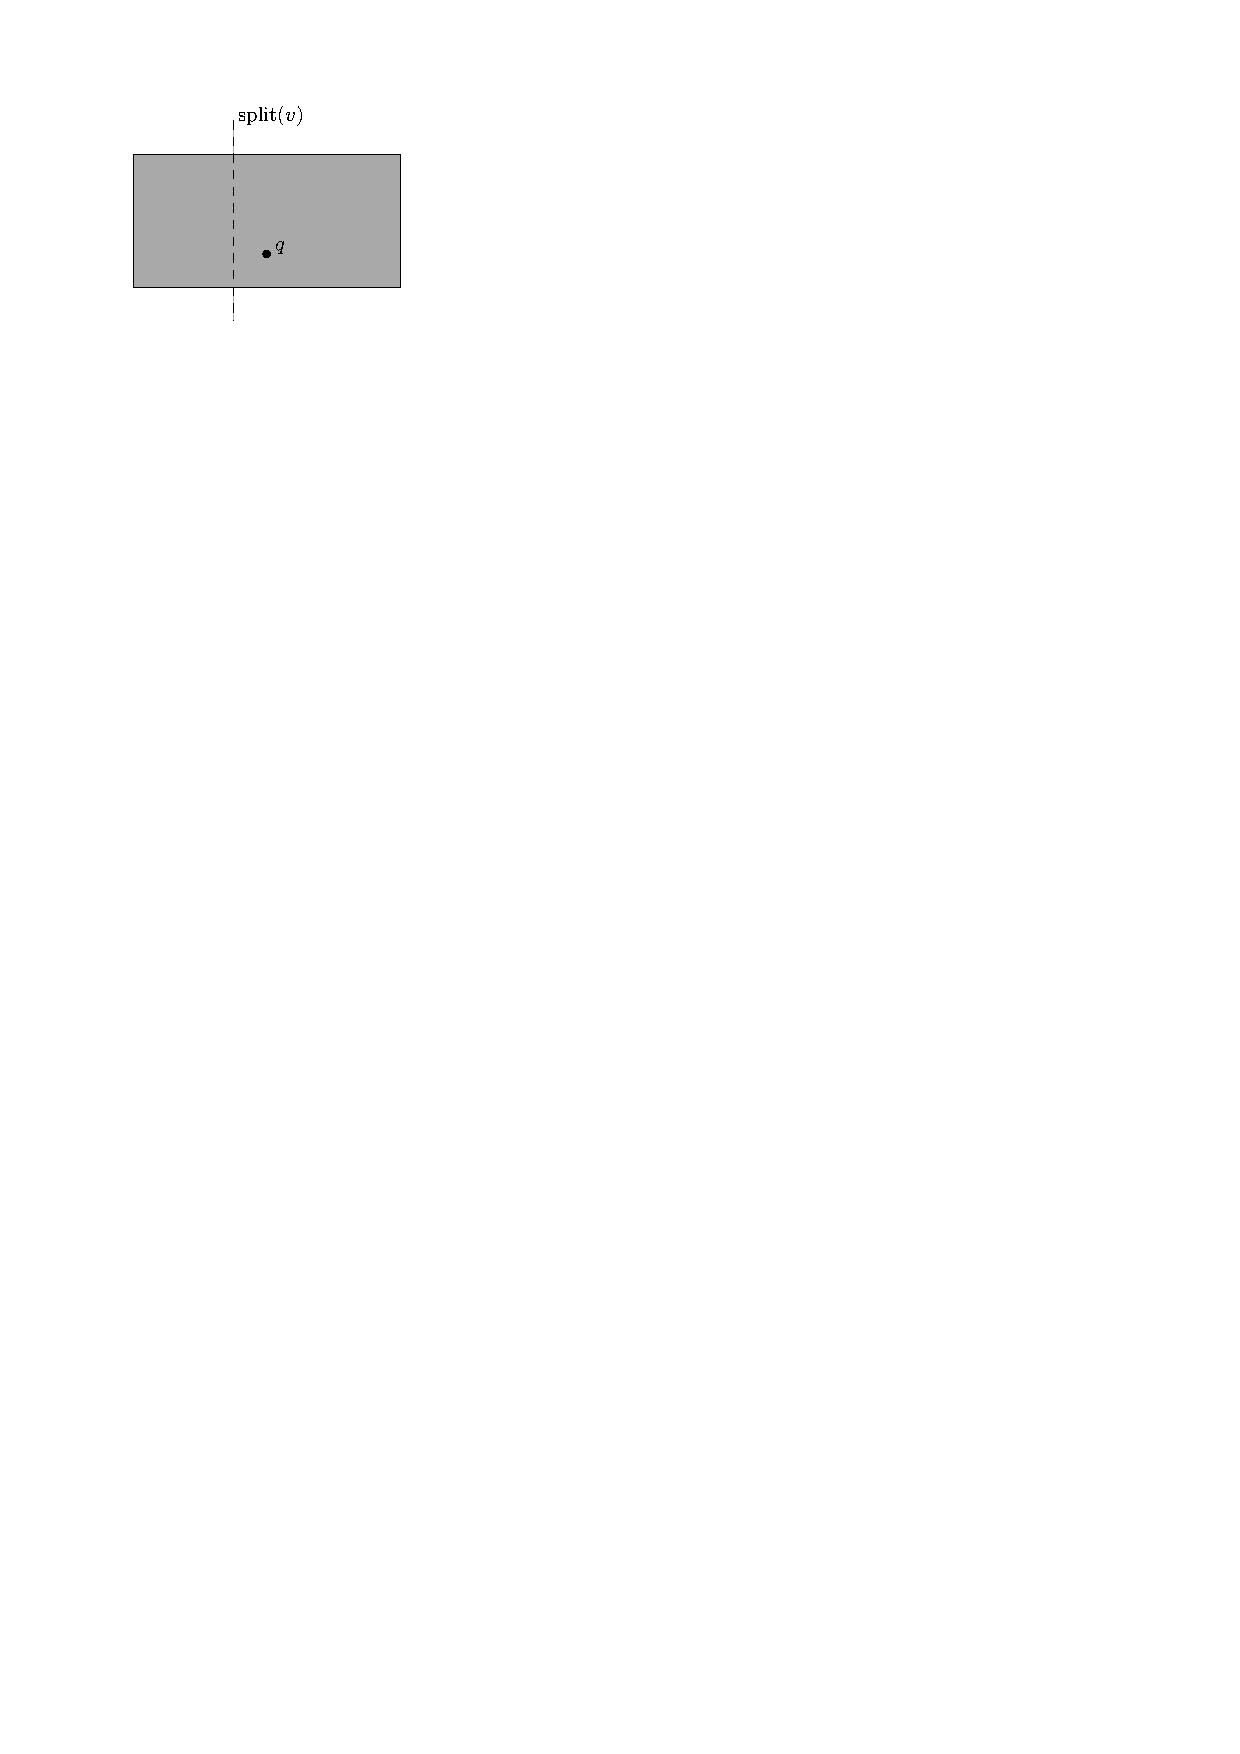
\includegraphics[width=0.20\textwidth,page=1]{figures/4-sided-to-3-sided}
  \caption[4-sided to 3-sided]{A 4-sided rectangle stored at $v$ is
    reduced to 3-sided rectangles on either side of $\splt(v)$ in an
    interval tree.}\label{fig:4sided:3sided}
\end{figure}

\section{\lspace{} 4-Sided: Faster with Near-Linear Space}
\label{sec:4sided}

Given two points $p,q \in \IR^d$, then $p = (p_1, \ldots, p_d)$
\emph{dominates} $q = (q_1, \ldots, q_d)$ if $p_i > q_i$ for all $i
\in \{1, \ldots, d \}$.  Given a set of points $P$, $R$ is a
\emph{$t$-level shallow cutting} of $P$ if
%
\begin{enumerate*}[label=(\roman*)] %chktex 36
\item $|R| = \BigOh{n/t}$,
\item any point $p$ that is dominated by at most $t$ points of $P$
  dominates a point in $R$, and
\item each point in $R$ is dominated by $\BigOh{t}$ points in $P$.
\end{enumerate*}
%
First, project the rectangles onto the plane.  Then build an interval
tree on the rectangles as we did in Section~\ref{sec:slow}, which such
that at each node $v$, our 4-sided projections are stored as 3-sided
rectangles either left or right of $\splt(v)$.  Consider each 3-sided
rectangle as a point, then we can take $\lg^{(i)} n$-level shallow
cuttings $R_i$ for all $0 \le i \le \lg^* n$.

\textbf{Local Structure} On each shallow cutting $R_i$, build the
structure from~\cite{afshani2008dominance}.

\textbf{Global Structure} Note that we can reduce dominance of a point
set $P$ in $\IR^3$ to planar point location in orthogonal subdivision
by projecting the orthants whose corners are at the points of $P$ onto
the plane, which we'll call the \emph{orthant projection}.  For each
$R_i$, compute the orthant projection $\mathcal{A}_i$, then store all
such projections in~\cite{chazelle1986filtering}.

To answer a query, first find all orthant projections which enclose
the query point by querying the global structure, then for each such
projection, query the local structure.

\textbf{Space} The local structure for each shallow cutting $R_i$
takes $\BigOh{n}$ space, and there are $\lg^* n$ such cuttings.

\textbf{Query Time} Querying the local structure takes $\BigOh{\lg^*
  n}$ time and is performed at each of the $\BigOh{\lg n}$ levels of
the interval tree.

\textbf{Remark} You can instead build a data structure with
$\BigOh{n}$ space and $\BigOh{\lg^{(c + 1)}n + k}$ query time by only
taking $c \ge 2$ shallow cuttings.

\begin{theorem}[3.1 in~\cite{saladi2015improved}]\label{thm:31}

  OPEQ on 4-sided rectangles can be answered using a structure of
  $\BigOh{n\lg^* n}$ size and $\BigOh{\lg n \cdot \lg^* n + k}$
  query time, where $k$ is the size of the output.

\end{theorem}

\section{\lspace{} 5-Sided: Putting it Together with Grids}
\label{sec:5sided}

We will use a grid technique adapted from~\cite{alstrup2000new}.  Let
$t = \lg^4 m$, where $m$ is the number of rectangles at the current
level of recursion (initially $n$).  Project $S$ onto the plane, then
draw an orthogonal $(2\sqrt{m/t})\times(2\sqrt{m/t})$ grid over the
resulting rectangles such that each horizontal and vertical slab
contains the projections of $\sqrt{nt}$ sides.  We create a tree by
creating a node to store all rectangles which cross a grid line, then
recurse on all other rectangles.  Stop recursion when $m$ reaches a
constant.  At each node of this tree:
%
\begin{enumerate*}[label=(\roman*)] %chktex 36
\item \emph{(slow)}: build the structure from Theorem~\ref{thm:21},
\item \emph{($L_c$)}: for each grid cell $c$, store at most $\lg^3 n$
  of the rectangles which completely cover $c$ in decreasing order of
  $z$ span, and
\item \emph{(side)}: build the structure from Theorem~\ref{thm:31} on
  the (at most 4) sides cut from each rectangle by the grid (see
  Figure~\ref{fig:grid:decomposition}).
\end{enumerate*}

To answer a query $q$, locate the grid cell $c$ containing $q$ and
scan $L_c$, reporting rectangles until
%
\begin{enumerate*}[label=(\alph*)] %chktex 36
\item\label{enum:a} we find a rectangle not containing $q$, or
\item\label{enum:b} we reach the end.
\end{enumerate*}

If~\ref{enum:b}, then $k \ge \lg^3 n$, thus querying the slow
structure gives $\BigOh{k}$ query time.  Otherwise, query the side
structures then the recursive structures.

\textbf{Space} The bottleneck is the structure from
Theorem~\ref{thm:31} which occupies $\BigOh{n\lg^* n}$ space.

\textbf{Query Time} The bottleneck is the recursive case.  Since we
can find the grid cell containing $q$ in $\BigOh{\lg n}$ time and the
size of the subproblem is $\sqrt{nt}$, we get $Q(n) = Q(\sqrt{nt}) +
\BigOh{\lg n}$.  With $t = \lg^4n$, this solves to $\BigOh{\lg n\lg\lg
  n + k}$ time, and this concludes the proof of Theorem~\ref{thm:51}.

\textbf{Remark} In the RAM model, we can find the grid cell containing
$q$ in $\BigOh{1}$ time.  This suggests we can achieve $\BigOh{\lg\lg
  n + k}$ query time.  Also, if Theorem~\ref{thm:31} is not the time
bottleneck, we can use the time-space trade-off to achieve $\BigOh{n}$
space.

\begin{figure}[t!]
  \centering
    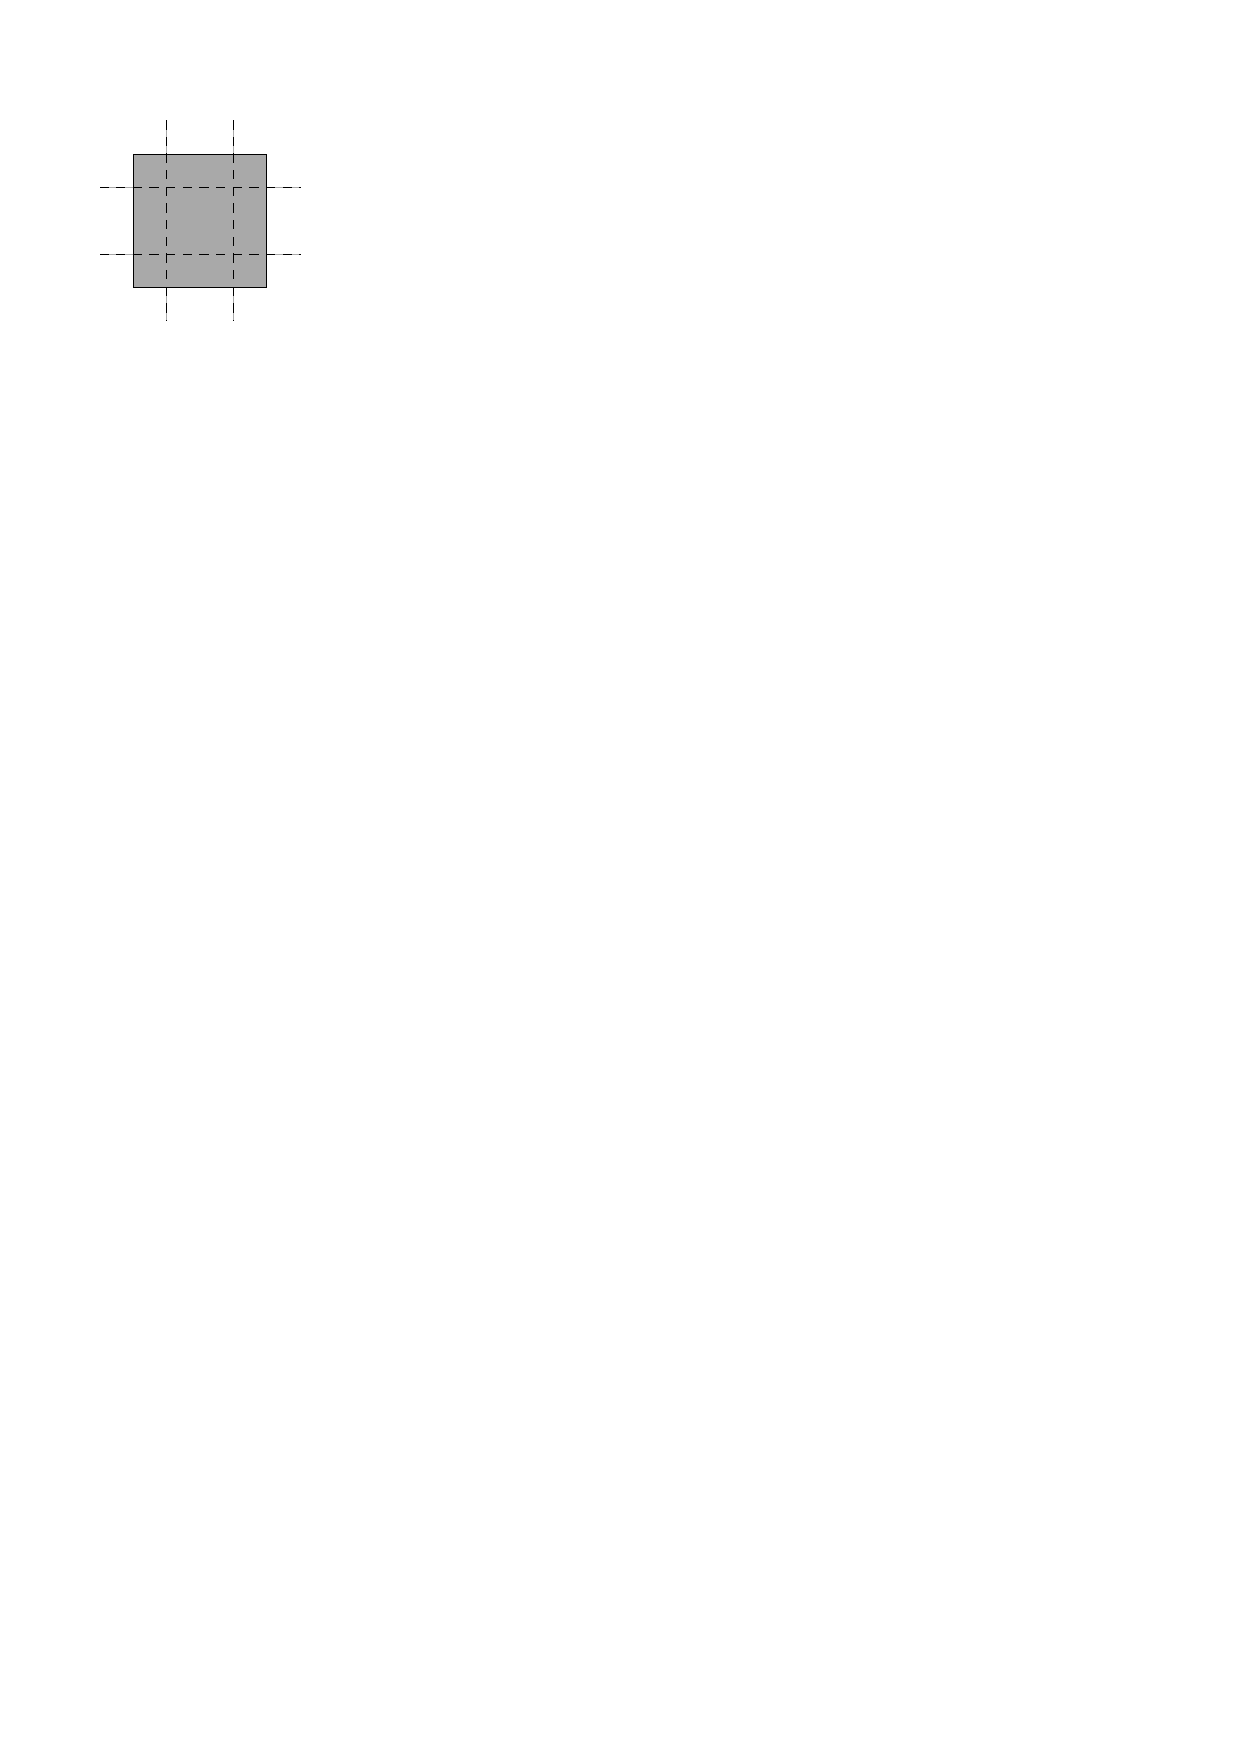
\includegraphics[width=0.10\textwidth,page=1]{figures/grid-decomposition}
    \includegraphics[width=0.10\textwidth,page=2]{figures/grid-decomposition}
    \includegraphics[width=0.10\textwidth,page=4]{figures/grid-decomposition}
    \includegraphics[width=0.10\textwidth,page=3]{figures/grid-decomposition}
  \caption[Grid decomposition]{A rectangle (left) decomposes into an
    number of totally covered cells (middle-left), sides contained in
    adjacent vertical slabs (middle-right), and sides contained in
    adjacent horizontal slabs (right).}\label{fig:grid:decomposition}
\end{figure}

\bibliographystyle{alpha}
\bibliography{Saladi-Notes-References}

\end{document} %chktex 17
